\documentclass[journal]{vgtc}                % final (journal style)
%\documentclass[review,journal]{vgtc}         % review (journal style)
%\documentclass[widereview]{vgtc}             % wide-spaced review
%\documentclass[preprint,journal]{vgtc}       % preprint (journal style)
%\documentclass[electronic,journal]{vgtc}     % electronic version, journal

%% Uncomment one of the lines above depending on where your paper is
%% in the conference process. ``review'' and ``widereview'' are for review
%% submission, ``preprint'' is for pre-publication, and the final version
%% doesn't use a specific qualifier. Further, ``electronic'' includes
%% hyperreferences for more convenient online viewing.

%% Please use one of the ``review'' options in combination with the
%% assigned online id (see below) ONLY if your paper uses a double blind
%% review process. Some conferences, like IEEE Vis and InfoVis, have NOT
%% in the past.

%% Please note that the use of figures other than the optional teaser is not permitted on the first page
%% of the journal version.  Figures should begin on the second page and be
%% in CMYK or Grey scale format, otherwise, colour shifting may occur
%% during the printing process.  Papers submitted with figures other than the optional teaser on the
%% first page will be refused.

%% These three lines bring in essential packages: ``mathptmx'' for Type 1
%% typefaces, ``graphicx'' for inclusion of EPS figures. and ``times''
%% for proper handling of the times font family.

\usepackage{mathptmx}
\usepackage{graphicx}
\usepackage{times}

%% This turns references into clickable hyperlinks.
\usepackage[bookmarks,backref=true,linkcolor=black]{hyperref} %,colorlinks
\hypersetup{
  pdfauthor = {},
  pdftitle = {},
  pdfsubject = {},
  pdfkeywords = {},
  colorlinks=true,
  linkcolor= black,
  citecolor= black,
  pageanchor=true,
  urlcolor = black,
  plainpages = false,
  linktocpage
}

\usepackage{subfigure}
\usepackage{flushend}
\setlength{\fboxsep}{0pt}

%% We encourage the use of mathptmx for consistent usage of times font
%% throughout the proceedings. However, if you encounter conflicts
%% with other math-related packages, you may want to disable it.

%% If you are submitting a paper to a conference for review with a double
%% blind reviewing process, please replace the value ``0'' below with your
%% OnlineID. Otherwise, you may safely leave it at ``0''.
\onlineid{103}

%% declare the category of your paper, only shown in review mode
\vgtccategory{System}

%% allow for this line if you want the electronic option to work properly
\vgtcinsertpkg

%% In preprint mode you may define your own headline.
%\preprinttext{To appear in an IEEE VGTC sponsored conference.}

\graphicspath{{figures}}


%% Paper title.

\title{Supporting Deep Brain Stimulation Interventions \\ by Fusing Microelectrode Recordings with Imaging Data}

%% indicate IEEE Member or Student Member in form indicated below
\author{Alexander Bock, Norbert Lang, Gianpaolo Evangelista, Ralph Lehrke, and Timo Ropinski}
\authorfooter{
%% insert punctuation at end of each item
\item
 Alexander Bock and Timo Ropinski are with the Scientific Visualization Group, Link{\"o}ping University, E-mail: \{alexander.bock,timo.ropinski\}@liu.se.
\item
 Norbert Lang and Ralph Lehrke are with the St. Barbara Hospital Hamm, E-mail: \{nlang,rlehrke\}@barbaraklinik.de.
\item
 Gianpaolo Evangelista is with the Sound Processing Group, Link{\"o}ping University, E-mail: giaev@itn.liu.se.
}

%other entries to be set up for journal
\shortauthortitle{Bock \MakeLowercase{\textit{et al.}}: DBS Visualization}
%\shortauthortitle{Firstauthor \MakeLowercase{\textit{et al.}}: Paper Title}

%% Abstract section.
\abstract{
Deep Brain Stimulation (DBS) is a surgical intervention, which is known to reduce or eliminate the symptoms of common movement disorders, such as the Parkinson's disease, dystonia, or tremor. During the intervention, the surgeon places electrodes within the patient's brain so that the regions responsible for the disease can be stimulated. Since these regions span only a couple of millimeters and electrode misplacement has severe consequences, reliable and accurate navigation is of great importance. Usually, the surgeon relies on fused CT and MRI data sets as well as feedback from the patient, who is not fully sedated during the intervention. More recently Microelectrode Recordings (MER), which support navigation by measuring the electric field of the patient's brain, are also facilitated. While MER has the potential to improve placement accuracy, the fusion with the available imaging data is performed by the surgeon through mental registration, which results in a higher cognitive load and potentially affects efficiency. To reduce the surgeon's cognitive load when applying MER, we propose an intra-operative visualization system which fuses multimodal imaging and MER data in an intuitive way. This fusion is achieved by {\it spatializing} the MER signal, which is usually analyzed in the time domain. We were able to design a multiview system, which supports DBS navigation by combining several 2D and 3D views to allow an intuitive registration of the space and the time domain. We will describe our design considerations, the technical realization, as well as the outcome of the proposed system.
}

%% Keywords that describe your work. Will show as 'Index Terms' in journal
%% please capitalize first letter and insert punctuation after last keyword
\keywords{Deep brain stimulation, multimodal visualization, multiple views.}

%% ACM Computing Classification System (CCS). 
%% See <http://www.acm.org/class/1998/> for details.
%% The ``\CCScat'' command takes four arguments.

\CCScatlist{ % not used in journal version
 \CCScat{I.3.7}{Computer Graphics}{Three-Dimensional Graphics and Realism}{Color, shading, shadowing, and texture}
}

%% Uncomment below to include a teaser figure.
%\teaser{
%\centering
%\includegraphics[width=16cm]{CypressView.eps}
%\caption{In the Clouds: Vancouver from Cypress Mountain}
%}

%% Uncomment below to disable the manuscript note
%\renewcommand{\manuscriptnotetxt}{}

%% Copyright space is enabled by default as required by guidelines.
%% It is disabled by the 'review' option or via the following command:
% \nocopyrightspace

%%%%%%%%%%%%%%%%%%%%%%%%%%%%%%%%%%%%%%%%%%%%%%%%%%%%%%%%%%%%%%%%
%%%%%%%%%%%%%%%%%%%%%% START OF THE PAPER %%%%%%%%%%%%%%%%%%%%%%
%%%%%%%%%%%%%%%%%%%%%%%%%%%%%%%%%%%%%%%%%%%%%%%%%%%%%%%%%%%%%%%%%

%\setlength{\fboxsep}{0.0mm}

\begin{document}

%% The ``\maketitle'' command must be the first command after the
%% ``\begin{document}'' command. It prepares and prints the title block.

%% the only exception to this rule is the \firstsection command
\firstsection{Introduction}
\label{sec:introduction}

\maketitle

%% \section{Introduction} %for journal use above \firstsection{..} instead
%
% As this stimulation has severe effects on the local function of the brain, placement accuracy is critical in order to prevent unwanted side effects. 
%
Due to the advances in medicine, society is now facing the problems of an aging population suffering from more and more age-related diseases. One such group of frequently occurring diseases are \emph{movement disorders}, such as Parkinson's Disease (PD), dystonia, or tremors, which greatly affect the patients', as well as their families' quality of life. As both, symptoms regarding the motor skills, as well as the psychological consequences of these diseases, have a great impact on everyday life, successful treatment strategies are of increasing importance.

Deep Brain Stimulation (DBS) is a well-established procedure for reducing the symptoms of these diseases~\cite{Lindberg2002,Yianni2003,Benabid2009}, and improving the overall quality of life in the cases where medication is not a viable option. To conduct a DBS, electrodes are implanted into specific regions of the brain, which then emit electrical signals designed to stimulate these regions. In the case of PD, the most effective target areas for electrode placement are the subthalamic nuclei (STN), which reach sizes of just a few millimeters~\cite{Richter2004} and are located symmetrically in both hemispheres. As misplaced stimulation electrodes can have severe side effects on the local functioning of the brain, such as speech difficulties and long term memory problems~\cite{Astrom2010}, accurate electrode placement is crucial~\cite{Rodriguez-Oroz2005}. Nowadays, the access path to the target region is most often planned by exploiting magnetic resonance imaging (MRI). Besides the low signal-to-noise ratio, a major downside of this imaging modality is, that the STN cannot be visually resolved with the required accuracy \cite{Starr2002}. Despite these problems, MRI based localization techniques are widely used, as they are the only mechanisms which enable to plan the access path pre-operatively. Thus, surgeons use an atlas-based approach to locate the STN within the MRI data. Obviously, this approach is prone to registration errors and lacks visual assessment. However, due to the lack of visual assessment, the patient is only partly sedated during the placement intervention, as the correct electrode positioning must be verified by testing the patient's movement, as well as speech and memory capabilities. Depending on the electrodes location, either temporary memory-loss, speech problems or a tremor increase indicates the position of the electrode. To further reduce the uncertainty of the electrode placement, besides these conducted patient tests, intra-operative x-ray scans are performed to check the electrode placement.

In recent years, Microelectrode Recording (MER) has emerged as a technique allowing the surgeon to better locate the target region for DBS intra-operatively~\cite{Lenz1988}. The interaction with the patient is nevertheless of great use, as it gives even more information about the position of the electrode than MER alone. MER measures the electrical field of the brain during surgery by inserting electrodes into the access path. These electrodes do not emit an electric field of their own, but measure the brain's electric field instead. The measured information is then used to differentiate functional regions and specifically the target region. In fact, a study conducted by Alterman et al. could show, that in 96\% of cases the intended target region was changed when applying MER~\cite{Alterman1999}. Another benefit is, that in contrast to x-ray scanning, this method does not use any ionizing radiation which should be, especially in the brain, avoided at all costs. While x-ray scans might still be performed after the surgery as a final check, MER has the potential to reduce the need for intra-operative scans. Though MER improves the accuracy of the intervention, it cannot be used to substitute the MRI scans, as they are still used to initially plan the access path. Only by combining MER data with the structural information acquired through MRI, the neurosurgeon is able to plan and perform all necessary steps during the DBS intervention. Furthermore, intra-operative patient checks do also not become obsolete, as their results allow to draw direct conclusions about the influence of the placed electrode. Unfortunately, current systems do not provide fusion of the structural and the functional modalities in an integrated way. In current systems, the MER signal is presented to the surgical staff by showing the amplitude in the time domain for each electrode similar to an oscillogram. On demand, the neurosurgeon can listen to an audible version of one signal in order to inspect it in detail. However, while the human visual memory is already limited, the capacity of the echoic memory is even lower, and its operations are more restrained, as humans do not process sounds sequentially, but as groups which are processed as one unit~\cite{Radvansky2005}. To overcome these memory limitations, surgeons have to perform frequent and repetitive measurements in order to mentally reconstruct the location of the target region from the brain's electrical field. Therefore, an expressive visual representation of the MER signal with the option of viewing the original data on demand, is desirable.

Within this paper, we propose an interactive visualization system, which exploits {\it spatialization} of the measured MER signal, and fuses it with imaging data and patient responses with the goal to reduce the cognitive load of the surgeon and thus improve the electrode placement during DBS. Instead of having the spatial and structural information, i.\,e.,~pre-operative CT, MRI scans, and intra-operative x-ray scans, inspected independently of the MER signal and the patient responses, we visualize this multimodal data in a single spatial context. This is beneficial, as it has been shown in other contexts, that presenting multiple modalities in an integrated manner can improve the information gathering process~\cite{10.1109/BIOMEDVIS.1995.10008}. In order to fuse the MER signal, given over time, with the spatial information, gathered from the scans, we employ a method to spatialize the MER signal. Furthermore, we provide the surgeon with a specialized view in which he can inspect the most probable target region, depending on the fused information. By visually overlapping the potential target areas, the surgeon can select a placement region with greater accuracy and certainty. Thus, our contributions are as follows:

\begin{itemize}
\item{A multimodal visualization system for performing DBS interventions.}
\item{An approach for the visual assessment of the most probable DBS target region, which fuses spatial and non-spatial data acquired from scans, MER measurements and patient checks.}
\item{Directions for designing future intervention systems, which have been derived from the evaluation we have conducted with five neurosurgeons.}
\end{itemize}



\section{Related Work}\label{sec:related}
%It was already shown in the introduction, that DBS is an established technique to reduce the symptoms of movement disorders \cite{Benabid2009}. Nevertheless, there is much research going on to further improve the effectiveness of this class of interventions. Since most of this research is done in the area of medicine, only two examples are presented here. One example of this research is \cite{McIntyre2006}, in which the authors describe the interaction between the electrode and the surrounding tissue by inspecting the volume of tissue activated as a function of the stimulation parameters. Another example is \cite{Butson2008}, in which this concept is taken further, so that not only the stimulation parameters are observed, but the geometric shape and number of the electrodes as taken into consideration as well.

%There have been a lot of studies which show that MER provides an improvement in electrode placement. Alterman~et~al.~\cite{Alterman1999} surveyed 132 pallidotomies and found that in 12\% of cases the actual target region was more than $4$mm apart from the intended target region. Ulbert~et~al. \cite{Halgren2001} proposed a system of recording multiple microelectrodes and provide a thorough description of the electronic details. One of the important works on the signal processing analysis of the MER, with regard to the differentiation of the target region, was done by Hutchison~et~al.~\cite{Hutchison1998}, when they examined 8 patients with idiopathic PD and analyzed the signals for different brain regions. They found that the STN could be identified by the presence of characteristic spike frequencies with irregular firing patterns. Benazzouz~et~al.~\cite{Benazzouz2002} confirmed this with 153 patients in a long-term study over the course of 9 years.

An important step in the DBS intervention consists of the trajectory planning, which is usually done manually. There has been a lot of work on (semi-)automatic trajectory planning in the last years. Chentanez~et~al. describe a method to avoid important structures with a rigid needle by simulating deformable tissue~\cite{Chentanez2009}. Gemmar et al. determine the mid-saggital plane and the localization of the anterior commissures (AC) and the posterior commissures (PC)~\cite{Gemmar2008}. Their method is based on a region-growing based segmentation algorithm, and requires a nonlinear anisotropic filtering kernel. The entry point is varied while for every trajectory a cost function is evaluated and the system operator selects the best trajectory. Bruneberg et al. facilitate a segmentation of the STN and determine the optimal trajectory by avoiding ventricles, gyri, and blood vessels, which need to be segmented beforehand as well~\cite{Brunenberg2007}. Khlebnikov~et~al. suggested a system to find optimal access paths by interpreting tumors as light sources and determining the cost-function based on that aspect \cite{Khlebnikov2011}. Another automated system for trajectory planning was proposed by Essert~et~al. who determined the optimal location and trajectory using geometric constraints \cite{Essert}. A visualization system for the pre-operative planning was provided by Beyer et al.~, who proposed a multi-volume renderer employing cut-away views to allow for visual access to the brain structures of interest \cite{Beyer2007}. Furthermore, they included a skull peeling algorithm, which we incorporated also in our system. Serra et al. propose a neurosurgery planning tool for tumor resections, which uses a virtual workbench to increase user immersion, and which provides additional 3D interaction tools~\cite{Serra1998}. Watanabe~et~al. developed a computer assisted surgery tool to treat cortical lesions and used a curvilinear reformatting to allow direct access to the data~\cite{Watanabe}.  More recently, Rieder et al. propose a planning tool for neurosurgical tumor treatment, which uses a cylindrical cut for a better view onto the target region~\cite{Rieder2008}. Additionally, they introduce a distance ring to denote the relative depth of a specific region of interest. Furthermore, the same authors introduce visualization techniques to enhance the perception of structures when using multimodal rendering setups~\cite{Rieder2008a}.

In the area of MER data integration, Miocinovic et al. provide a system for a guided DBS electrode implantation in non-human primates~\cite{Miocinovic2007}. They provide metaphors for visualizing region information, but base the information only on a 3D atlas, instead of the MER signal. As no patient checks can be performed, a combination of potential target regions is not employed. Furthermore, their main focus is a MER-based region detection for generating an atlas of the brain. D'Haese et al. present a system for the use in human surgery~\cite{Haese2005}, but they focus more on the comparison between MER selected targets and atlas-based target selection. They also do not incorporate the patient test information into their system, which is required for a sufficient level of accuracy and confidence. Sperka et al. also present a system to improve the planning phase for computer-aided stereotaxic surgery planning~\cite{Sperka2011}. They focus on the planning phase of the entry point and determining the trajectory alone. Furthermore, the use of fMRI data together with other modalities was investigated in the context of stereotactic interventions on macaques~\cite{Ohayon2012}.



\section{Microelectrode Recording}\label{sec:mer}
\begin{figure}
    \centering
    \subfigure[Thalamus]{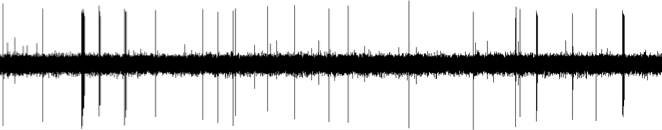
\includegraphics[width=0.49\columnwidth, height=0.17\columnwidth]{figures/Thalamus.png}}
    \subfigure[Zona incerta]{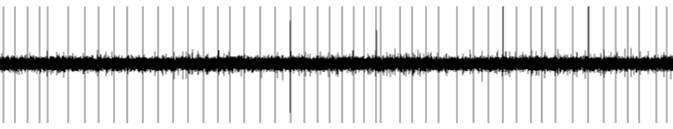
\includegraphics[width=0.49\columnwidth, height=0.17\columnwidth]{figures/Zona_incerta.png}}\\
    \subfigure[Nucleus subthalamicus]{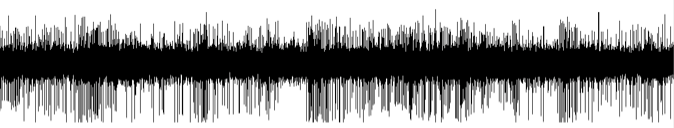
\includegraphics[width=0.49\columnwidth, height=0.17\columnwidth]{figures/nucleus_subthalamicus.png}}
    \subfigure[Substantia nigra]{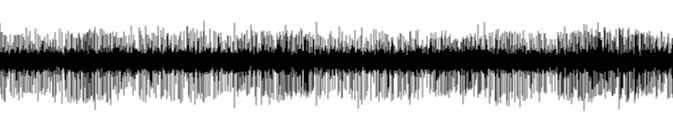
\includegraphics[width=0.49\columnwidth, height=0.17\columnwidth]{figures/substantia_nigra.png}}
    \caption{The MER discharge pattern changes depending on the functional region of the brain. The level of background activity and single-cell activity varies when entering or leaving specific regions, and can be used to clearly identify these region~\cite{Benazzouz2002,Hutchison1998}.}
    \label{fig:dischargepatterns}
\end{figure}

MER is an intra-operative technique to gain information about functional areas of the brain, which are referred to as nuclei. This information is gathered by inserting electrodes, which measure the electric field properties created by the discharge of individual neurons in the surrounding tissue~\cite{McIntyre2006}. In the human brain, there are a number of different types of neurons which each have a distinct discharge behavior. The combination of those types in a nucleus leads to detectable discharge patterns, which can be used to identify the region in which the measurement electrodes are located. Figure~\ref{fig:dischargepatterns} shows examples of the signals acquired from different brain regions. One possibility to distinguish the nuclei is to analyze the frequency of spikes within these signals. Usually, this information is presented to the surgeon as an audio signal, an oscillogram, and as the result of a simple frequency analysis, e.\,g., a power density function. Based on this information, the neurosurgeon can identify the current region and decide on how to proceed with the intervention. Different MER setups exist for measuring the electric fields. The system we used to record the data used in this paper contains five electrodes with a square geometry, whereby the fifth electrode is located in the center and the sides measure $1.5$mm.

%As systems with different numbers of electrodes and geometries are available, our system is designed to handle different geometries and different numbers of electrodes. In order to prevent any confusion from the start, we chose to model the visual representations of the electrodes in such a way, that it is not consistent with any commercially available system. Otherwise, there might be the possibility that a surgeon recognizes our electrode representations of being type A, while they are in fact type B. Since he might deduct certain aspects from a specific electrode type, this mistake must be prevented.



\section{System Overview}\label{sec:overview}
\begin{figure*}[t]
    \centering
    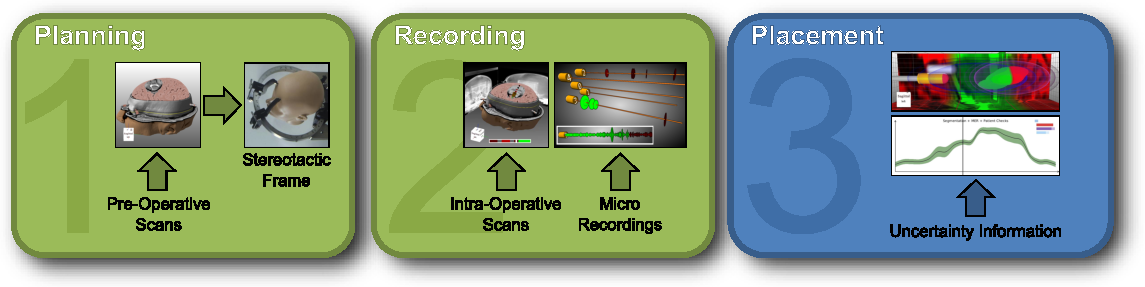
\includegraphics[width=0.9\linewidth]{figures/workflow}
    \caption{The workflow of the proposed visual DBS intervention system can be divided into three phases: planning, recording and placement. To support each of these phases, we employ dedicated views which are arranged in a multiple view setup. External components interacting with our visualization system are shown for each phase.}
    \label{fig:workflow}
\end{figure*}

The main goal of the designed system is to increase the efficiency and, more importantly, the effectiveness of the neurosurgical team during DBS interventions, by fusing the available modalities and thus facilitating mental registration~\cite{Tory1998}. The current situation in the operating room is, that the methods for inspecting the structural modalities, i.\,e.~MRI, CT, and biplanar x-ray scans, are fairly advanced and widely used. However, the system for recording and analyzing the MER signals is usually decoupled from the other modalities. It is a stand-alone unit which has no connection to the anatomical structures or visualization parameters and vice versa. Furthermore, the results of the patient checks are not accounted for in a formalized manner.


\subsection{DBS Intervention Procedure}\label{sec:overview:procedure}
Before proposing our system, which has been designed to improve the current situation, we will first give a high-level overview of the DBS intervention procedure, as it is specified in surgery guidelines~\cite{Hemm2010}. With respect to the subparts of this procedure, a DBS intervention can be roughly divided into three subsequent phases:

\begin{itemize}
\item \textbf{Planning phase.} During this phase, the surgeon selects the intended target region and determines an optimal trajectory to access that region. We will describe how this phase is supported by the proposed system within Section~\ref{sec:overview:planning}.
\item \textbf{Recording phase.} In this phase, the measurement electrodes are inserted into the brain, and moved towards the intended target region, while the electric field around them is recorded. This data is analyzed and the MER-based target region estimation is derived as described in Section~\ref{sec:overview:recording}.
\item \textbf{Placement phase.} After determining the target position based on neuroanatomical features, and narrowing them further down using the MER measurements, the stimulating electrode is inserted into the target region, and the patient's cognitive and motor functions are tested, to get a more accurate estimate of the target region and find the optimal placement position. We describe the parts of our system dedicated to this process in Section~\ref{sec:overview:placement}.
\end{itemize}

As these three phases define the overall workflow of a DBS intervention, they are used as the blueprint for the workflow underlying the presented visualization system (see Figure~\ref{fig:workflow}). However, to enable accurate navigation and data handling between the phases, more details about the DBS intervention procedure need to be considered.

As accuracy is of uttermost importance when performing DBS interventions, the patient is mounted into a stereotaxic frame, which is rigidly fixed to the patient's skull (see inset in the planning phase in Figure~\ref{fig:workflow}). This frame has sockets, which hold and precisely guide the equipment used during the intervention. An important property of the frame is, that it is visible in both, CT and MRI scans, and thereby serves as one of the landmarks used in the registration process. Thus, the surgeon can plan the target region based on the pre-operatively acquired T$_1$ and T$_2$ MRI scans. Nevertheless, in most cases the target region is not directly visible on either of the MRI scans, and the surgeon has to rely on experience and guidelines to locate the target area. In the case of the STN, this is done as follows. First, the Talairach coordinate system is created based on the AC and PC regions, which are easily identifiable in MRI data~\cite{Talairach1993}. After defining this patient-specific Talairach coordinate system, a patient-neutral heuristic is used to find the STN target region relative to one anchor point, e.\,g.,~the PC. After identifying the target region, the surgeon determines the entry point which minimizes the amount of critical structures, e.\,g.,~blood vessels or active areas of the brain, in the straight line between those. All these steps are performed within the planning phase of the DBS intervention. We will describe the visualization metaphors, which we have developed to support this phase in Section~\ref{sec:overview:planning}.

\begin{figure}[b]
    \centering
    \subfigure[Anterior-Posterior]{\fbox{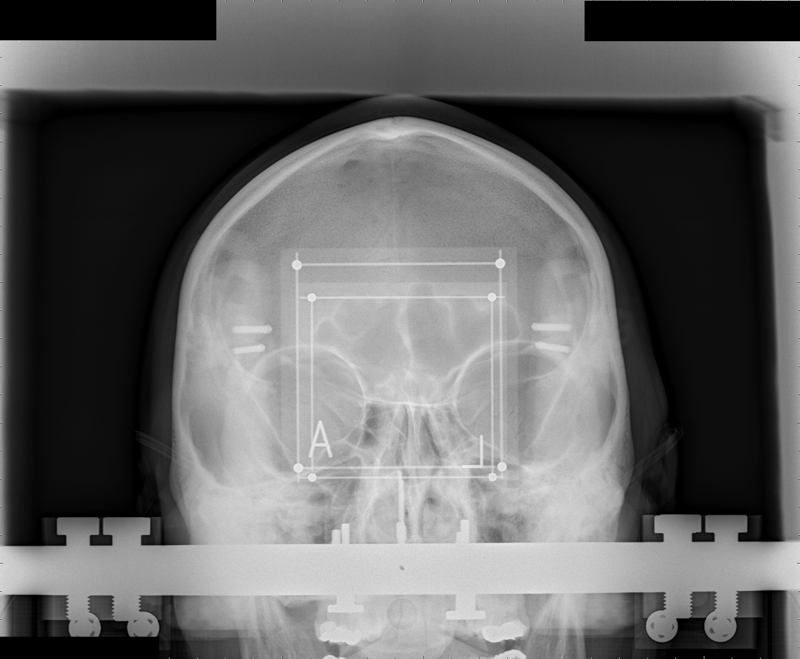
\includegraphics[height=0.45\linewidth]{figures/xrayslice-ap.png}}}
    \hspace*{0.2cm}
    \subfigure[Dorsal-Ventral]{\fbox{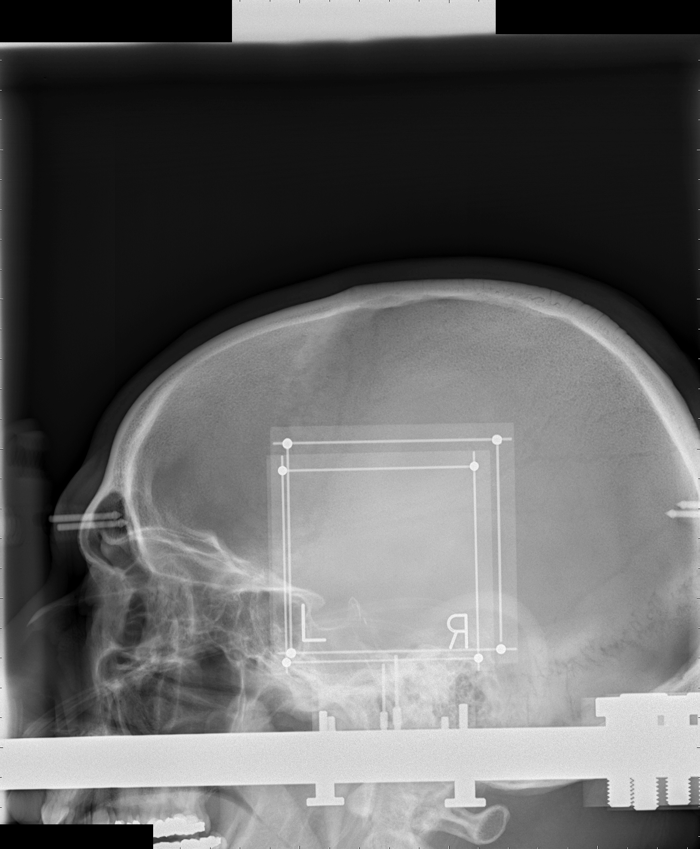
\includegraphics[height=0.45\linewidth]{figures/xrayslice-dv.png}}}
    \caption{Two x-ray images are created to calibrate the patient's position in the operating room using the perspective distortion of the reference plates. Subsequent x-ray images are used to verify the electrodes position inside the head.}
    \label{fig:xrayreferencescans}
\end{figure}

Besides the pre-operative MRI scans, also a pre-operative CT scan is made, and at the beginning of the intervention, two orthogonal reference x-ray scans are acquired (see Figure~\ref{fig:xrayreferencescans}) to support registration of the x-ray coordinate system and the patient. As shown in Figure~\ref{fig:xrayreferencescans}, two wireframe plates with a known geometry are mounted on the stereotaxic frame to support this registration. Once the x-ray scans have been acquired, the skull is opened and the MER electrodes are inserted, such that the recording phase can be started. During this phase, the electrodes are moved forward towards the intended target region, while they continuously record the discharge pattern. During this procedure, one member of the surgical team observes the resulting signal, analyzes it and informs the surgeon. The electrode movement is controlled through a micrometer motor, which allows for precise movement and localization of the electrodes. The micrometer motor is attached to the stereotaxic frame and the needle containing the MER electrodes is inserted into that motor. The depth values are calibrated and measured in such a way, that they indicate the distance to the intended target location in a micrometer scale. As soon, as the target location within the STN is reached, its depth is stored and the electrodes are retracted again. We describe the developed visualization techniques supporting the recording phase in Section~\ref{sec:overview:recording}.

After the MER electrodes have been removed, the stimulating electrode is inserted into the micrometer motor and the electrode placement is performed. Upon reaching the target depth, the electrodes are activated and start emitting, at which point the surgeon-patient interaction begins. The surgeon tests the patient's cognitive and motor functions in order to further narrow down the optimal electrode location. The patient's speech, motor, and memory capabilities are tested here. To monitor and verify this process, orthogonal x-ray scans are obtained. We describe the visualization techniques developed to support the placement phase within Section~\ref{sec:overview:placement}. As these techniques show the data acquired before and during the intervention in a fused way, they can also be used to review the operation in a long-term, vertical, follow-up study. Then, over a long period of time, the cognitive and motor functions of the patients could be tested and rated. Ideally, the physician would want to perform a horizontal study as well, in which he can correlate the planned target location, the MER-corrected target location and the level of improvement to each other. This would allow to iteratively improve the heuristics, the surgeons use for DBS placements and potentially lead to improved success rates.


\subsection{Planning Phase}\label{sec:overview:planning}
The goal of the planning phase is to identify the desired target region based on pre-operative scans, and to plan a trajectory reaching that target region by minimizing the distance to critical structures along the access path. There are a number of highly specialized tools available to perform this task, and there is also active research in the field of automatic trajectory planning~\cite{Shamir2010}. Since our focus in this system is on the intra-operative parts of the procedure, we implemented a basic planning tool, which bridges the gap between the pre-operative scans and the presented visualization techniques. This allows the surgeon to transfer the results of external planning tools into our integrated system. This transfer requires two subsequent steps. First, the target region is selected on a slice representation of the MRI scan. Second, the entry point of the trajectory is selected in a 3D multimodal visualization of the pre-operative scans. Figure~\ref{fig:planningphase:view} shows the setup of the two incorporated views with both, the target point and the entry point selected. As the 3D view contains all contextual information relevant during each phase of the DBS intervention procedure, it is used within all phases and serves as a red thread through the phases of the system.


\subsubsection{Slice View}\label{sec:overview:planning:slice}
\begin{figure}
    \centering    
    \subfigure[Slice View \label{fig:planningphase:slice}]{\fbox{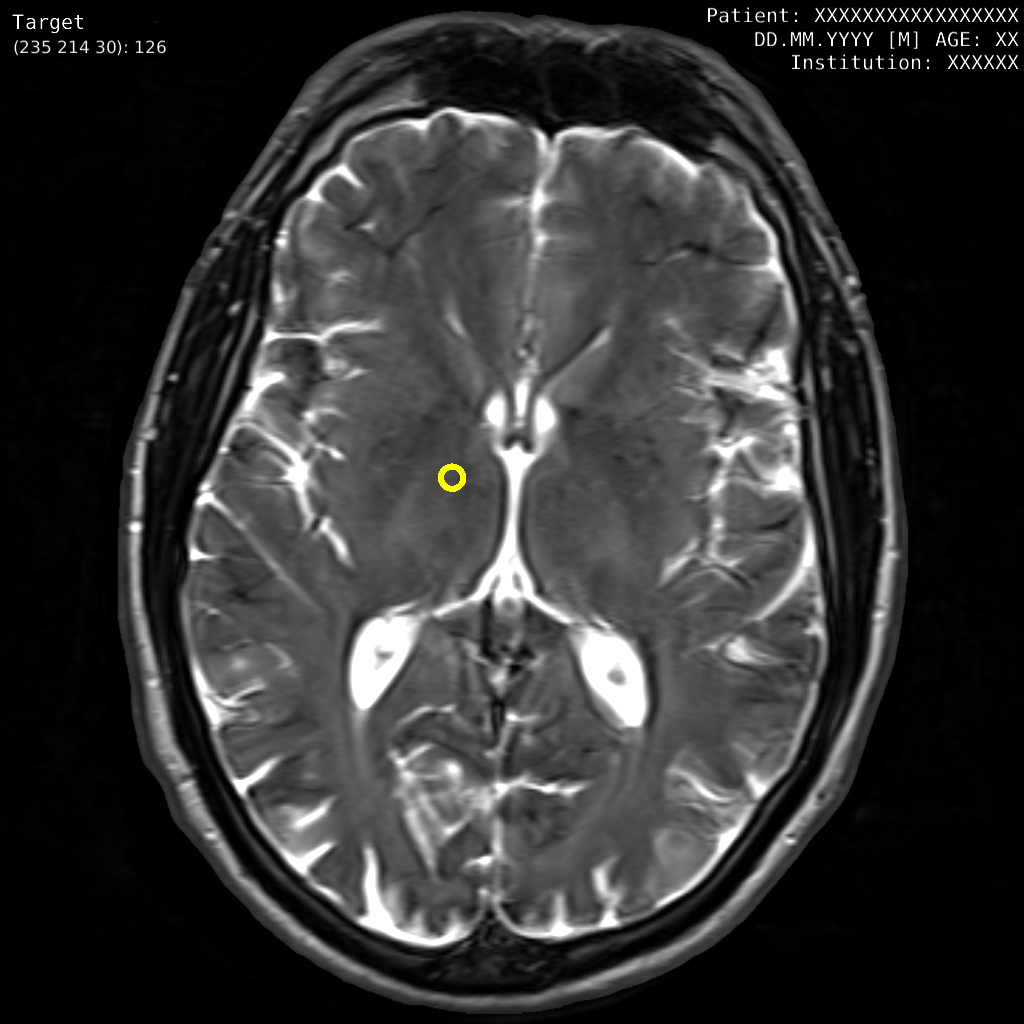
\includegraphics[width=0.49\columnwidth, height=0.49\columnwidth]{figures/planning-slice}}}
    \subfigure[Contextual View \label{fig:planningphase:3d}]{\fbox{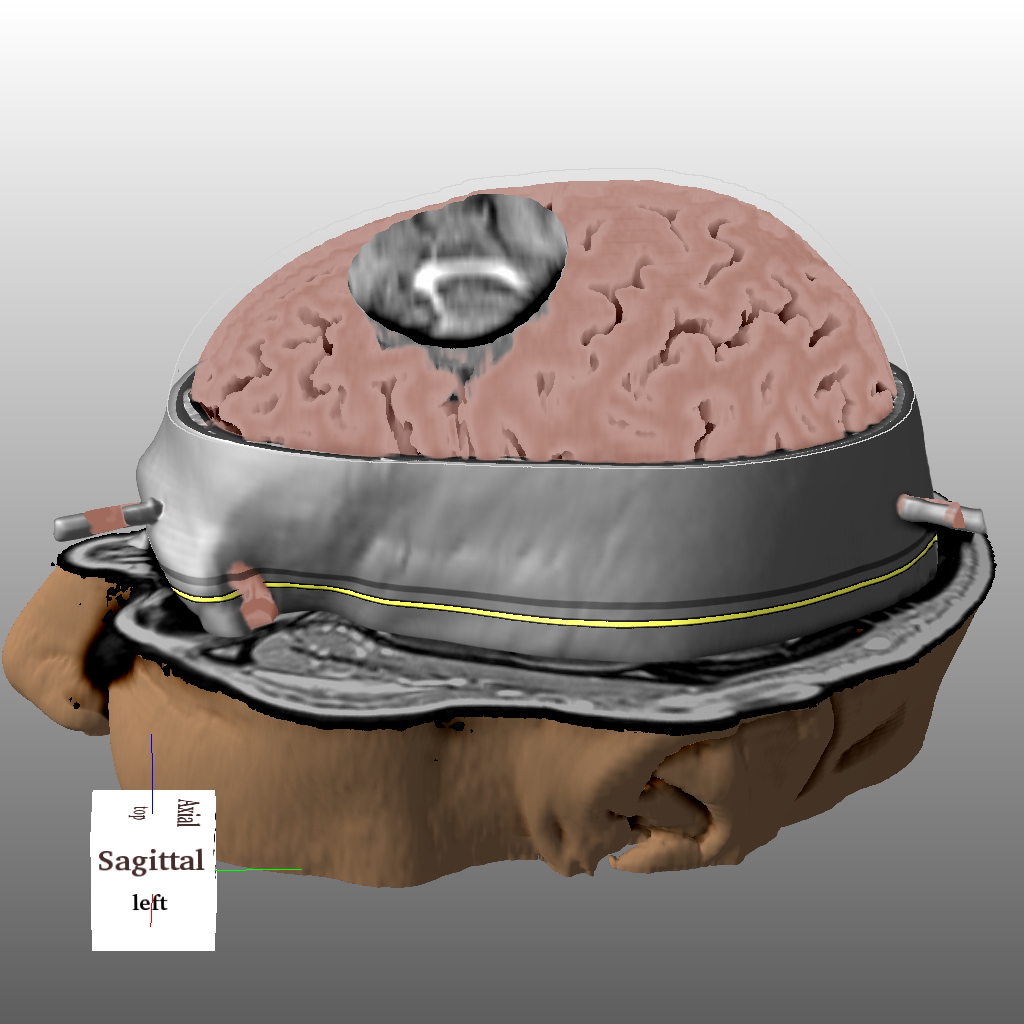
\includegraphics[width=0.49\columnwidth, height=0.49\columnwidth]{figures/planning-3d}}}
    \caption{During the planning phase, two linked views are employed. A slice view helps to select the target region (a), while a linked contextual view helps to interactively define the minimal invasive access path (b).}
    \label{fig:planningphase:view}
\end{figure}

In the slice view (see Figure~\ref{fig:planningphase:slice}), the surgeon can browse through the slices of the two pre-operative MRI scans. Thus, this rather standard view allows for determining the probable location of the target region and identifying it at a sub-voxel accuracy. Even though the pre-operative MRI scans are acquired at high resolution, the sub-voxel accuracy is crucial for accurate electrode placement, as the target region given by the STN spans only a few millimeters. Therefore, the neurosurgeon can pan and zoom within this slice view. Furthermore, the view presents the user with information about the intensity value at the selected point and the patient's information in the upper right hand corner. The color of the marker in this view was chosen to provide a good contrast with the MRI signal, and allows mental registration with the slice indicator shown in the contextual view.


\subsubsection{Contextual View}\label{sec:overview:planning:3d}
The contextual view is the common element that is present during all three phases of the proposed system. This constant present is useful, as it creates a \emph{horizontal mental registration} between the different phases in addition to the \emph{vertical mental registration} present within each phase. The latter is achieved by using this view as a frame of reference so that the individual information of the other views can be related to the common contextual view. The contextual view qualifies to be used for this mental registration purpose, as it displays all relevant information in a fused manner.

The contextual view is based on a multimodal visualization of the pre-operatively acquired CT and MRI scans. To improve spatial comprehension, the three modalities are not entirely fused, but vertically separated such that for each region the modality of highest interest is visible (see Figure~\ref{fig:planningphase:3d}). At the bottom, we render the T$_1$-weighted MRI with a transfer function that shows the whole head of the patient. The T$_1$ modality was chosen, because it allows for an easier classification of the skin using the spin-lattice time compared to the spin-spin time, and second, the relatively stable gradients allow for reasonable shading. Nevertheless, in principle when no T$_1$ MRI is available, this part could also be substituted by a T$_2$ scan. However, as we fuse this part with a slice representation of this modality, CT would not be optimal as it has a low brain contrast. This part rather helps to communicate the orientation of the patient, as left-right mismatches would be crucial, then the actual anatomy. The cut-off line between this region and the upper one can be interactively moved by the user to allow for data inspection. The cut-off of the lower region is caped with a slice view having the same properties as the main slice view described in Section~\ref{sec:overview:planning:slice}. Thus, this slice serves as an easily identifiable visual element, which further improves the vertical mental registration. Furthermore, it provides the surgeon with direct access to structural information embedded within a spatial context. To obtain an occlusion-free view to the brain, which is the main structure of interest, we employ an interactive skull stripping approach above the cut-off, which is described in greater detail in Section~\ref{sec:implementation}. As MRI has a low signal-to-noise ratio and the skull stripping might not be faithful to the brain surface for all points, gradient-based shading is not an option when visualizing the brain. Instead, we employ depth darkening~\cite{Luft2005}, which results in a rather natural representation of the brain and thus provides a good spatial overview. As mentioned above, the contextual view is additionally linked to the target area selected in the slice view, by projecting a yellow slice indicator onto the visible structures. This view further includes an inset view which provides a clear orientation regardless of the view direction to help the mental registration even further.

As it is not possible for the surgeon to physically look onto the target through the opening in the skull during the operation, it is often helpful to virtually increase the diameter of the access path and thus remove the structures around the trajectory~\cite{Weiskopf2002,Rieder2008}. The removed area is cylinder-shaped and possesses a variable, user-defined radius, such that the surgeon can inspect the walls of cylinders with varying radii to gain more insight. To increase the amount of information the surgeon gains from the cylinder walls, the same transfer function as used in the slice representations, is applied here. This increased access path radius gives the surgeon access to more information in a spatial context, which he could not have gained otherwise.

So far, all the described features of the contextual view are common to all three phases. However, the specialty in this phase for the contextual view is, that it also indicates the slice which is currently viewed in the slice view, as a dark gray band projected onto the head. Based on this band, the surgeon can immediately see at which depth the currently viewed slice is located. While any surgeon will possess the knowledge to infer this information from the surrounding tissue or by comparing the number of total slices to the current slice number, both methods require conscious or subconscious mental processing, which should be avoided. Perceiving a band projected to the 3D structures is a much more intuitive way requiring almost no cognitive effort, such that the surgeon can focus on locating the target region.


\subsection{Recording Phase}\label{sec:overview:recording}
The recording phase is the next step during a DBS intervention, following the opening of the patient's skull. While moving them deeper towards the target region, each of the electrodes detects the signals from the surrounding tissue and transmits them to the controlling device. To obtain knowledge about the current region, the received signals are constantly analyzed and classified. This phase consists of the following views: the Contextual View provides the necessary mental registration and provides a coherent frame for the other views, the Multi-Planar Slice View gives information about the immediate area surrounding the electrodes, and two audio representations enable analyzing the recorded signal. We could have included the Electrode Closeup (see Section~\ref{sec:overview:placement:targetareaview}) in this phase as well, but this view needs information from the patient interaction which will be acquired only later in the procedure.

\subsubsection{MER Signal Analysis}\label{sec:overview:recording:signalanalysis}
The MER signals are highly corrupted by noise, as the transmission is followed by an amplification of around three orders of magnitude, i.\,e.,~from $\mu V$ to $V$, which introduces $1/f$ wideband random component noise. In our system, also another type of noise was detected, a set of sinusoidal or very narrow band signals pitched at constant frequencies. While the $1/f$ noise is justified by thermal noise in the amplification system, which reaches critical levels, the origin of the sinusoidal components is unknown and probably due to interference with other equipment used during surgery. The $1/f$ noise has amplitudes comparable to the neuron pulses to be detected, while the latter are still audible in the auditory analyses.

In order to better condition the signal for audio analysis and thus for visualization, we tapered the amplitudes of the sinusoidal noise components. This was achieved by means of a set of notch filters tuned at the frequencies of the sinusoids. In order to reduce the impact of the denoising process, we decided to eliminate only the most prominent sinusoidal components. Sinusoidal tapering was achieved as follows. First, the frequencies of the sinusoids were detected by means of a peak picking algorithm, then a set of band stop Type I Chebyshev filters were designed, one for each frequency. In order to guarantee the stability of the design and effectively eliminate the sinusoidal components, we found it optimal to use filters of order six, with a stop band margin of $1\%$ of the sampling rate and stopband centered at the detected frequencies of the sinusoids, and ripple of $0.1$ dB. The neuron firing signal being wideband guarantees that the introduction of small band gaps has no other acoustical impact than reducing discomfort and distraction due to the presence of the sinusoids. Since the $1/f$ noise and the neural firing signals are both wideband and have comparable amplitude, we did not attempt direct removal of this noise component, in the effort of minimizing the deterioration of the signal. Other methods have been proposed for the same means~\cite{Jansen,Donoho1995}, but we found our method to be sufficient for the handled recording data.

In the target region, the amplitude of the neuron firing signal is higher than that of the noise floor. For automatic detection and visualization purposes a threshold on the noise floor is estimated in zones where the neuron firing signal is not present. Applying this threshold to the instantaneous signal amplitude in the time domain has then the effect of revealing and enhancing the peaks of the neuron firing signal when they are present. Based on this signal, possibilities exist to automatically detect the region. However, the analysis and computation of these metrics is not in the main focus of this paper so this it is not elaborated on in detail. Instead, any of the following variants can be chosen, and a comparative study might be the focus of future work. One possible set of metrics consist of the firing rate, burst index, pause ratio, and the pause index, which were introduced by Haese et al.~\cite{Haese2005}. They also determined, that these metrics are useful to map the signals to specific brain regions. These values are computed using the denoised signal and applying a non-linear energy operator as presented by Maragos et al.~\cite{Maragos1993} and a spike detection with a subsequent thresholding presented by Mukhopadhyay et al.~\cite{Mukhopadhyay1998}. Other comparable approaches exist and it makes no systematical difference for our setup, which of the classification algorithms are used.


\subsubsection{Contextual View}\label{sec:overview:recording:3d}
\begin{figure}
    \centering
    \fbox{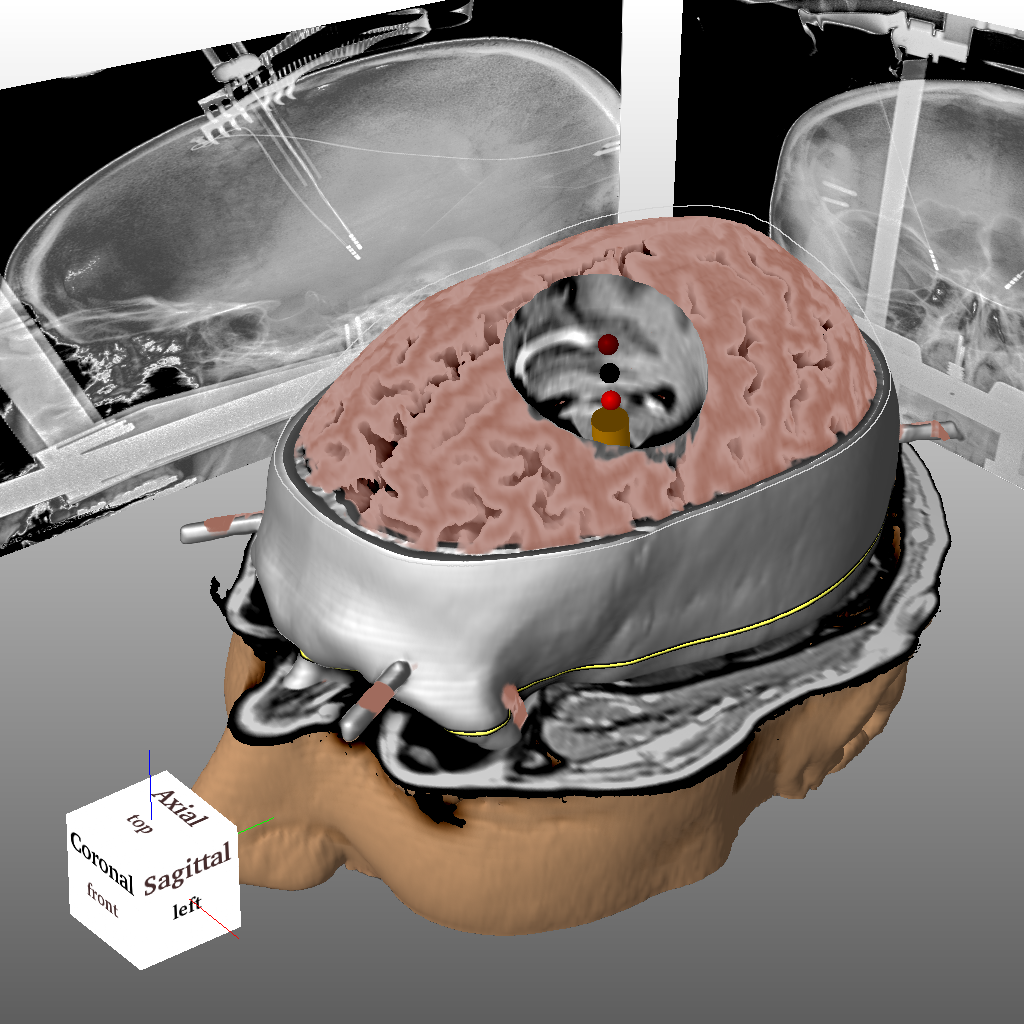
\includegraphics[width=0.9\columnwidth]{figures/recording-3d}}
    \caption{In the recording phase, the contextual view additionally shows the intra-operatively acquired x-ray scans. It further shows the electrode while it is advanced towards the target. The beads behind the electrodes show the results of the MER signal analysis in an intuitive way, and are also used for mental coregistration between different views.}
    \label{fig:recordingphase:3d}
\end{figure}

The contextual view as employed in the recording phase is in most parts identical to that one used in the planning phase, discussed in Section~\ref{sec:overview:planning:3d}, as it should provide the horizontal continuity between the different phases. However, as this phase of the intervention process requires additional information, the view differs in some ways. First, since the current depth of the MER electrodes is known and we know the entry point and the target region, we can compute and display a representation of the electrodes. Since the extent of the electrodes is very small compared to the whole head (see Section~\ref{sec:mer}) and we are only interested in the general position of the electrodes, just a single representative proxy electrode is visualized. 

Using the MER signal analysis from the previous section, we can classify depth values by their functional areas. Doing this continuously for every point along the trajectory would introduce a lot of visual clutter into the rendering, which would not give additional insight but rather confuse the user. Therefore, we classify and summarize segments along the trajectory, which we can classify up to an acceptable certainty. For each classified segment, we display a visual representation, which we refer to as a \emph{bead}, of this point in the center of the canal at that specific position. Each bead is rendered as a shaded sphere with a specific color. This visual metaphor has been proposed before~\cite{Miocinovic2007,Haese2005}, and provides both contextual and functional information simultaneously. The bead color indicates which type of tissue was classified around the position at which the bead is located. A black bead is created if there has been a longer distance without a reliable classification. These intermediate beads are important to maintain the geometric analogy of a bead string, which helps the user in understanding the spatial relationship between those. Different shades of red are used for areas, which lie out of the desired target area. Even though the detected areas are not the target region, it is nevertheless important to present this information to the surgeon, as he might deduce more information from the changes between different areas. The first choice for a color would be different shades of gray, but since the canal wall is gray and the human visual system is not adapted to differentiate gray tones, we chose red as the hue for these regions. As soon as the analysis of the spike signals  indicated that the MER electrodes are in the target region, green beads are rendered, which draws preattentive attention to those structures. Furthermore, this color coding resembles the traffic light color scheme proposed by Rieder et al.~\cite{Rieder2010}, that intuitively assigns green to {\it good} areas, while red is assigned to {\it bad} areas. To further reduce visual clutter, only one bead is rendered for all electrodes. This is a viable simplification, as the different functional regions of the brain are oriented such that either all electrodes detect the same signal (either type of tissue or undefined), or a subset of electrodes detects a regional signal and the others detect an undefined signal, in which case we use the defined signal.

Even with the application of the depth darkening shading technique described by Luft et al.~\cite{Luft2005}, the depth perception of the electrode is not optimal. One possible solution is the introduction of a distance ring as described by Rieder et al.~\cite{Rieder2008}. To reduce occlusion within the focus of the view, we decided to visualize a linear scale outside of the view's focus. Thus, this depth widget is located at the bottom of the view, where it does not block any relevant structures. The vertical white bar in this scale gives immediate feedback about the electrode's position. This widget is the first visualization used within our system, which employs a \emph{normalized view}. That means, that the left-most position correlates to the entry point at the skull's surface and the right-most position is the intended target region. As soon as a functional area has been detected, as described in the previous section, the background of the tube is filled with this color as well. Even though the beads convey a good absolute spatial orientation, their relative orientation is not immediately obvious because of occlusion and perspective distortion. On the other hand, the distance widget does not contain any information about the absolute spatial orientation. The combination of the beads in the contextual view and the color in the distance widget provide the relevant information to the surgeon.

Another addition to this view is the inclusion of the intra-operative x-ray images, which can be easily registered to the patient using the external and internal camera matrices and the known geometry of the two reference plates~\cite{Caprile1990,Zheng2008,Hartley2004}, which are shown in Figure~\ref{fig:xrayreferencescans}. As these x-ray scans are used to guide the surgeon on his way to the target region and provide one important possibility to verify the final position of the electrode, the integration with the other spatial modalities is important.


\subsubsection{Multi-Planar Slice View}\label{sec:overview:recording:mpr}

\begin{figure}[t]
    \centering
    \fbox{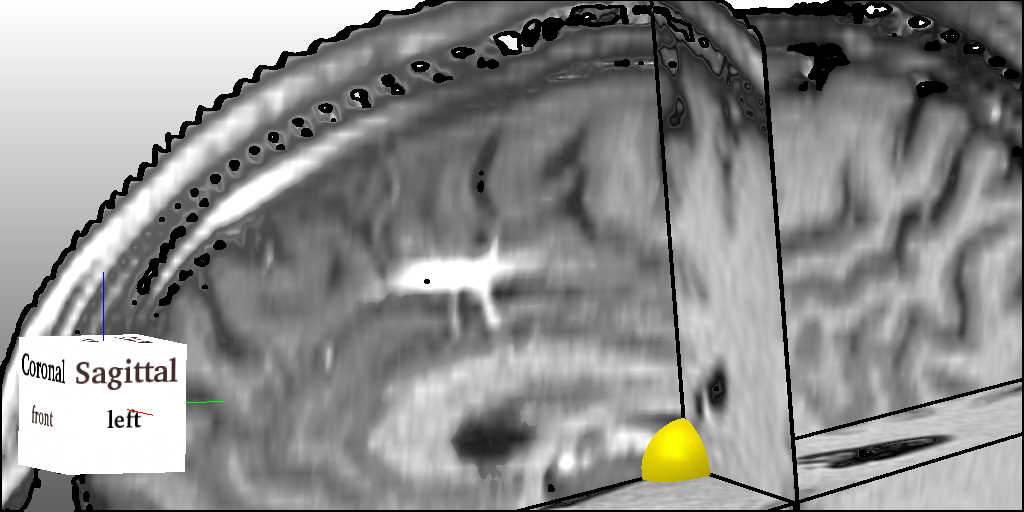
\includegraphics[width=\columnwidth, height=0.35\columnwidth]{figures/recording-mpr}}
    \caption{The Multi-Planar Slice View shows the position of the MER electrodes in the context of the surrounding tissue. The orthogonal slices are oriented so that one plane caps off the canal and another lies in the midsaggital plane, while the third plane is perpendicular to the other two. The intended target region resides in the intersection of the three planes and is represented by a small sphere. The current position of the electrodes is shown by a disc in the same color as the electrodes.}
    \label{fig:recordingphase:mpr}
\end{figure}

The multi-planar slice view shows three orthogonal slices centered on the intended target region. Its main purpose is to allow a better occlusion-free depiction of the current's electrode position and orientation in relation to the planned target region. The beads are visible in this view as well, but in addition to the other views in which they are present, each electrode's signal is analyzed on its own. This way, the surgeon can inspect the different analyses of the signals in more detail and can gain deeper insight. To depict the electrode placement, a disc is shown at the current electrode's tip position. As this disc communicates the current position, the size of the tip and the beads are not crucial in this view, and can thus be enlarged for better identification. While this enlargement results in an increased occlusion, this poses no problem, as identification of structures around the electrode is performed in the detail view discussed further below.

The slices of the multi-planar slice view lie in the coordinate system defined by the the canal axis, the midsaggital plane, and the cross product of those. To reduce the degree of occlusion introduced by the opaque slices, two of the slices are clipped, such that irrelevant regions are discarded. This, among others, focuses the user's attention on the central structure of the image, which contains the intended target region. The third sagittal slice is not clipped, in order to preserve the structure context as well as coherency with the contextual view.


\subsubsection{2D Temporal Audio Visualization}\label{sec:overview:recording:mer}
\begin{figure}[b]
    \centering
    \fbox{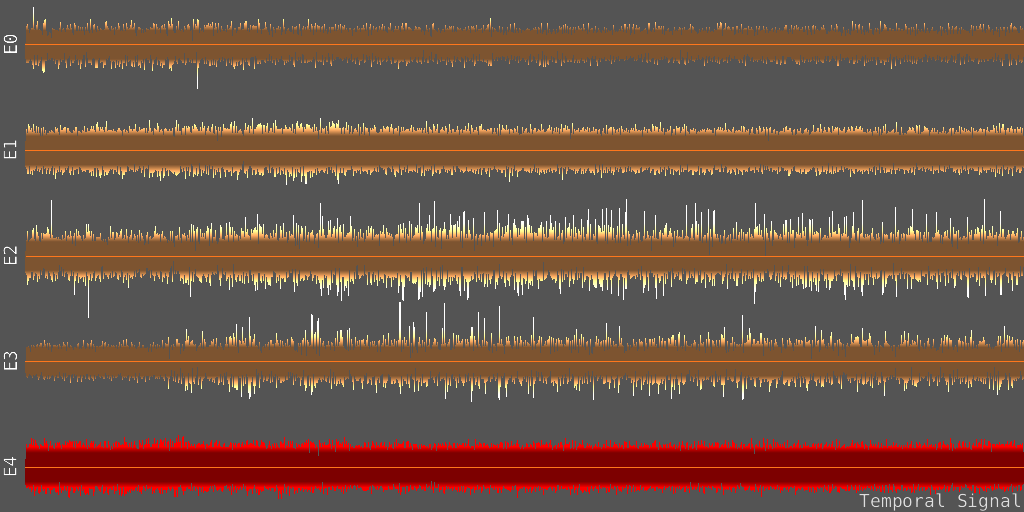
\includegraphics[width=\columnwidth, height=0.35\columnwidth]{figures/recording-sound.png}}
    \caption{To visualize the MER signal in the time domain, we use an oscillogram-like representation, in which time is on the horizontal axis with the new signals appearing on the right and the electric potential difference is shown on the vertical axis. The visual perception of the signal is enhanced by deemphasizing the background noise and guiding the attention to the more important spikes. The signal of the currently selected electrodes is highlighted.}
    \label{fig:recordingphase:sound}
\end{figure}

In this view, we present the raw data collected by the MER electrodes in real time. Since our recording setup consists of five electrodes, five graphs are visible, where each shows the amplitude (vertical axis) plotted over time (horizontal axis). The center line denotes an electric potential difference of $0V$. Even though the output data is in the order of $\mu V$, the actual values can vary between different commercially available systems, such that the scaling of the y-axis can be manually adjusted. On the left hand side next to the graphs are the identifying names for each electrode, as specified through the electrode geometry.

Since surgeons are generally more interested in the distribution of spikes than the background noise, we visually enhance spikes, such that they are the immediate focus of attention. This visual enhancement is done by defining a threshold value, below which all values are deemphasized, i.\,e.,~a darker color is chosen, and above which the values are emphasized with a brighter color. There is an exponential transition in the area around the threshold to reduce any unwanted attention, which would could otherwise result from discontinuities. This threshold value can be varied by the user to include a wider or narrower range of values in the focus area. The color scheme, which was used, matches the color on the electrodes and at the same time intensifies the perceptual distance between the colors used for the threshold area and the spikes.

Furthermore, to facilitate linking between all views containing a representation of the MER signal, the surgeon can select electrodes which are then automatically highlighted in all views (see Figure~\ref{fig:recordingphase:sound}). A problem with current systems is, that the surgeon must maintain a mental model relating the horizontal oscilloscope graphs with the geometric orientation of the electrodes within the patient's head. By creating a linked view between those two representations, we reduce the mental burden on the surgeon even further without preventing him access to any of the information.


\subsubsection{3D Temporal Audio Visualization}\label{sec:overview:recording:3daudio}
\begin{figure}[t]
    \centering
    \fbox{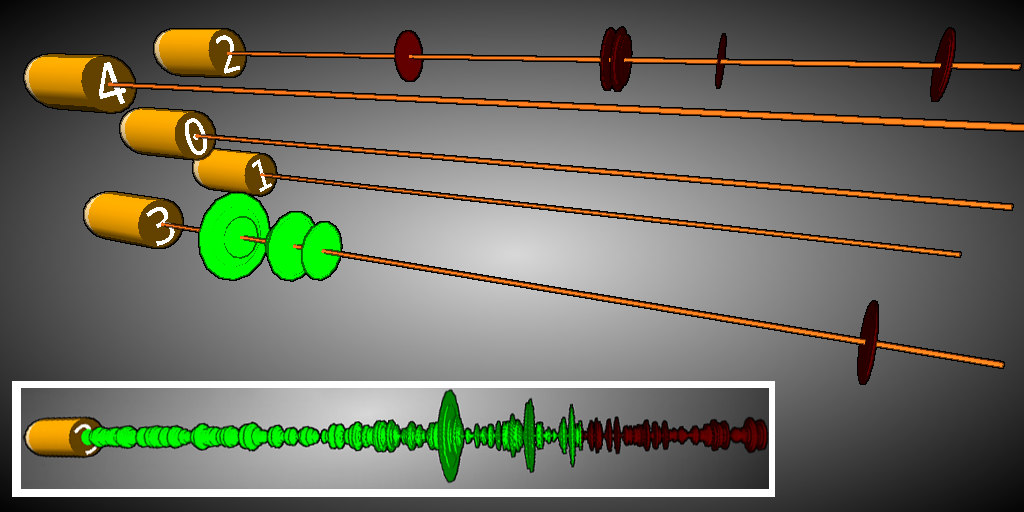
\includegraphics[width=\columnwidth, height=0.4\columnwidth]{figures/recording-3dsound}}
    \caption{Fusing the spatial orientation and layout of the recording electrodes with the temporal signal relieves the surgeon of the burden to keep this association in mind. To enhance the perception of the spikes, only the values above a certain threshold are shown in this view so that they are visible pre-attentively. The picture shows the same signal for subsequent time steps. The inset shows the result for one electrode without thresholding.}
    \label{fig:recordingphase:3dsound}
\end{figure}

As one of the key components of the presented system is a spatialization of the MER signal, it is important to bridge the gap between the MER signal defined over the time domain and the structures contained in the imaging data. We achieve this bridging, by employing a 3D temporal audio visualization, that directly combines the structural information of the electrodes with their temporal electric signal. The electrodes follow the camera movement of the contextual view but remain oriented in the way they actually are within the patient. This creates another element of mental registration between this view and the others. This way, the surgeon does not need to keep the orientation of the electrodes in mind and can more easily relate the structural information with the MER time domain. 

In addition to the structural information also present in the multi-planar slice view, each electrode shows its electric signal as concentric discs around the centerline. The discs start at the back end of the electrode with a radius, which is linearly connected to the absolute value of the amplitude. As soon as the next measurement is registered, the discs move away from the electrode and a new disc is inserted at the back end. This way, the signal originates from the electrode and moves away from it over time. Considering the absolute value of the amplitude is sufficient, as the spikes are distributed symmetrically and surgeons are not interested if the spikes occur because of a negative potential difference or a positive one.

Creating a disc for every measurement point clutters the whole view (see inset in Figure~\ref{fig:recordingphase:3dsound}), which is why we apply the same thresholding technique as described in the previous section. In this case however, we discard all signals which lie below the threshold. In the 2D case, the color was used to separate the thresholded values but since we only keep the spike values, we can use the results of the analysis from Section~\ref{sec:overview:recording:signalanalysis} to color and shade the visualized discs.


\subsection{Placement Phase}\label{sec:overview:placement}
In the placement phase, the surgeon needs to consider all acquired information to decide on the optimal position of the stimulating electrode. This decision is based on five different factors, the first being his experience and knowledge by selecting the intended target region during the planning phase. Second, the results of the MER recording and the area along the trajectory, which is likely to be the target region with respect to this data. The other three factors are acquired when the stimulating electrode is inserted and activated. The surgical staff will test the patient's cognitive and motor functions. These tests are beneficial, because it is well-known which areas affect which mental capabilities when being stimulated. From this information, the surgeon can further narrow down the location of the optimal target region, and the placement can be synchronized with the intra-operative x-ray scans. To aid in this final phase, we provide the surgeon with five different linked views. In contrast to the recording phase, where there were five recording electrodes, the surgeon only inserts a single stimulating electrode in the placement step, so that only a single electrode is presented in each view.

Again, the contextual view introduced above is shown to maintain the surgeon's mental registration. However, since the whole trajectory has been measured in the previous phase, all beads and all information previously acquired in the canal tube is presented independent of the electrode position. 


\subsubsection{Spatial Audio Visualization}\label{sec:overview:placement:spatialaudio}

\begin{figure}[t]
    \centering
    \fbox{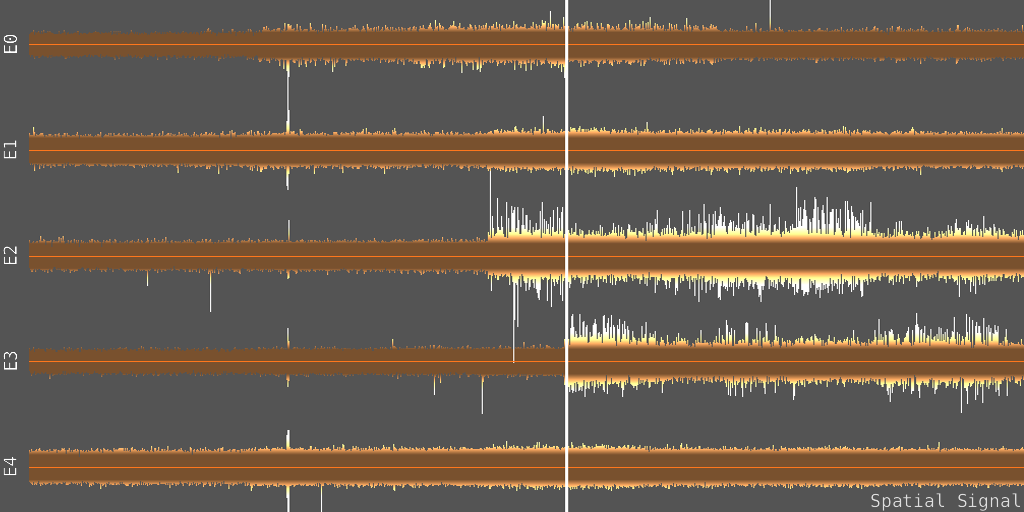
\includegraphics[width=\linewidth, height=0.4\columnwidth]{figures/verification-sound.png}}
    \caption{For the placement phase, it is necessary to inspect the MER signal based on the location where it was recorded, rather than depending on the time. This view is a normalized view, which shows the entry point on the left and the desired target region on the right. The visual enhancement is not as extensive as in Figure~\ref{fig:recordingphase:sound} since the preattentive perception is not as important here.}
    \label{fig:placementphase:spatialsound}
\end{figure}

The spatial audio view presents an overview over all the data points which were measured by the electrodes, such that it behaves similar as the temporal audio visualizations discussed above. The important difference, however, is that this graph does not plot time against amplitude, but rather position, i.\,e.,~depth vs. amplitude. The view is normalized similarly to the distance widget, so that the entry point lies on the left end of this view, while the target region is on the right side. Alternatively, this signal can be skewed in such a way, that the deepest electrode position is shown on the right. Although, this makes the mental registration with other views, where the target region forms the right border, more difficult, it also gives temporary access to the recorded data past the target region.

Similar to the temporal audio visualization, a modifiable threshold is applied to highlight the spikes and make them easily distinguishable from the background noise. This has a special importance in this view, since the surgeon inspects all values at the same time and might miss important data because of the visual clutter which would be otherwise visible.


\subsubsection{Canal View}\label{sec:overview:placement:canal}

The canal view provides access to information about the tissue surrounding the planned trajectory (see Figure~\ref{fig:placementphase:canal}). It is a normalized view with the entry point on the left side and the target region on the right, such that mental registration is easily possible with the spatial audio view. The canal view is generated by casting rays from a cylinder surface centered on the trajectory to another centered cylinder surface. The canal view is generated through regular volume raycasting, whereas the entry and exit points have been modified to fit the cylindrical geometry. Thus, the image of dimensions $X$ and $Y$ is a 2D presentation of the cylinder points in polar coordinates. That means that the axis of the cylinder is subdivided into $X$ concentric rings, with each vertical point representing an angle of $2 \pi / Y$. This way of presenting the area surrounding the trajectory allows the surgeon to analyze the data occlusion free, and into all directions simultaneously. In order to create the vertical mental registration, the current depth of the electrode as well as the detected regions are shown as overlays. The regional overlays are just thin stripes instead of areas, so that they do not occlude any detail which is shown below. To further explore the structures surrounding the access path, the diameter of the two cylinders used to generate the canal view can be varied. 


\subsubsection{Electrode Closeup}\label{sec:overview:placement:targetareaview}

\begin{figure}[b]
    \centering
    \fbox{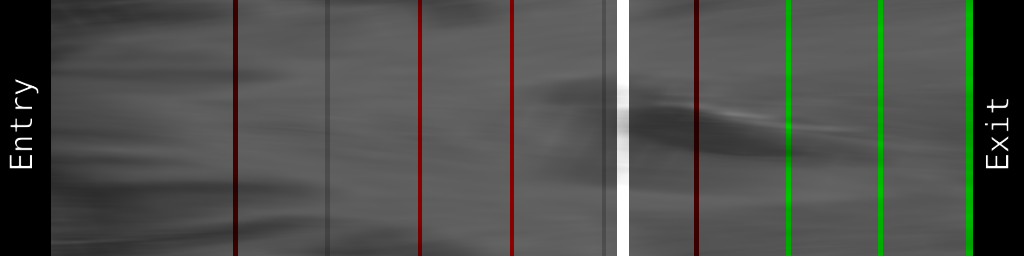
\includegraphics[width=\columnwidth, height=0.2\columnwidth]{figures/verification-canal.png}}
    \caption{The canal view presents the surgeon with a representation of the tissue within a cylinder centered on the trajectory. This allows for occlusion-free inspection of the MRI signal in all directions simultaneously. The current depth of the electrode and the analysis of the MER signal are shown as an overlay to provide easy registration.}
    \label{fig:placementphase:canal}
\end{figure}

\begin{figure}[t]
  \centering
  \fbox{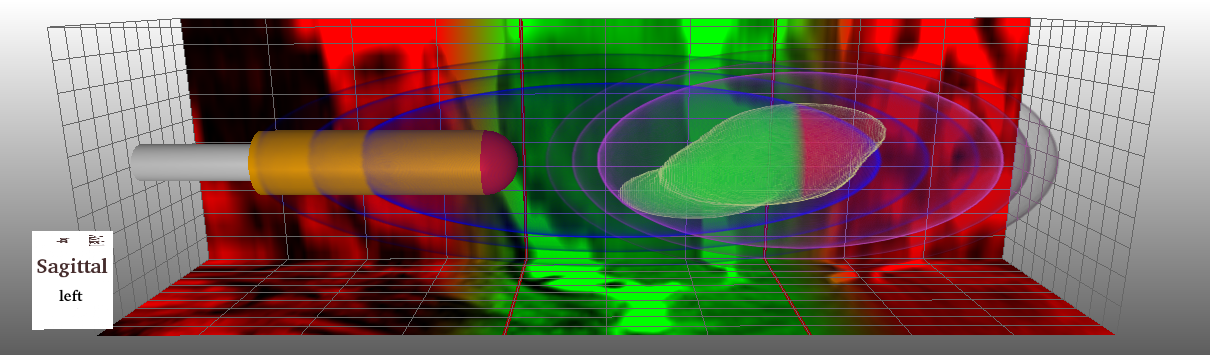
\includegraphics[width=0.98\columnwidth]{figures/target-region_intersection}}
  \fbox{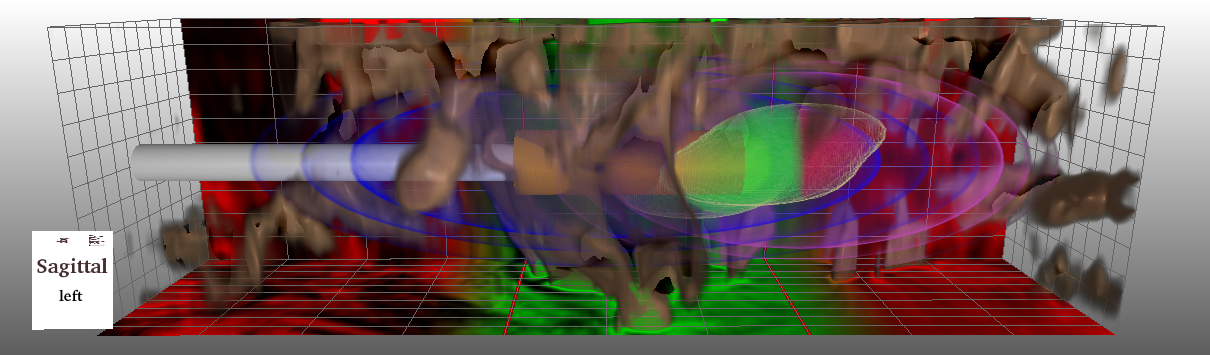
\includegraphics[width=0.98\columnwidth]{figures/target-region_full}}
  \caption{The electrode closeup visualization shows the potential target regions (planned=yellow, speech tests=blue, movement tests=purple). Furthermore, the spatial context provided by the MRI signal is color coded using the red-green MER region mapping. The electrode changes color when it is entering the intersection of the potential target area, and the spatial 3D context can be blended out to reduce occlusion.}
  \label{fig:targetregion}
\end{figure}

As accuracy is important when performing the electrode placement, the surgeon must be able to see where exactly the electrodes are located during the measuring process as well as the insertion process. This localization procedure must not only enable communicating the electrode position with respect to anatomical structures, but also with respect to the desired target regions which are obtained through patient tests and MER recordings. An optimal placement of the stimulation electrode should be in the intersection of the potential target regions obtained from the different measurements. We support this in-detail navigation aspect by providing a 3D visualization, which shows the electrodes embedded within the potential target regions. We refer to this visualization as the electrode closeup, as it shows details about the environment where the electrode is currently located. During the recording phase, this customizable view shows the five probing electrodes, while it presents the single stimulation electrode during the placement phase. To support the placement process, up to five potential target regions and their intersection are shown in a fused manner. These potential target regions are: the pre-operatively planned one using the MRI data, the one derived from the MER measurements, and the ones derived from the patient tests, i.\,e., speech, memory and movement. To relate these potential target regions to the electrode and embed them into the spatial context, we additionally display the pre-operative MRI scans. This is done in two different ways, ones as an optional 3D visualization, and once as a view-dependent projection on the back faces of the electrode closeup's bounding box. The 3D visualization has been made optional, as it on the one hand can provide valuable information regarding the intersection between the electrode and structures of interest, but on the other hand also occludes the potential target regions. The same orientation overlay is used in the electrode closeup, which is also used in the other 3D representations, to allow a seamless embedding of this view.

We have to deal with three different types of potential target regions, whereby the type of a region depends on the way it has been acquired. First, the planned region, which has been manually defined by the surgeon on the basis of the pre-operative MRI scan. As this process can be considered as a manual segmentation, the shape of this type of region is rather arbitrary. The second type of potential target region is derived from the MER signal. As all five electrodes filling out the entire access path have been used for the signal acquisition, the distinction between segments belonging and not belonging to the potential target region can be assumed as constant with respect to the radius of the access path. The third type of potential target region, i.\,e., those which are derived from the patient tests, have yet another shape as they have been derived from the tests performed when placing the actual stimulation electrode, which has only a single tip and thus does not entirely fill-out the access path defined through the measurement electrodes. Consequently, a specific visualization method, which enables communication of these different shapes, is needed for these three region types. Furthermore, it must be possible to depict the intersection of these differently shaped regions, as this intersection is the best possible estimate of the final target region. As the patient checks are conducted during the electrode placement phase, the corresponding regions should further be changeable interactively. Finally, in order to account for registration misplacements and other uncertainty sources, an uncertainty margin should be added to each of the visualized regions.

As the image-based target region specification basically resembles a segmentation process, which can have an arbitrary shape as outcome, we can apply volume rendering to show the result of this planning process. Since this segmentation is manually performed by the surgeon prior to the intervention, and it is based on the pre-operative MRI scan shown as the spatial context, the placement of this region is not subject to registration errors. We therefore usually set the uncertainty margin to zero in this case. This is different when visualizing the potential target regions acquired during the patient checks. As electrode tracking uncertainties with respect to image data registration may result in slight displacements, an uncertainty margin is required. As such a potential target region can be based on several patient checks, which are performed during the intervention, we assemble them by connecting several check points which then form an ellipsoid in 3D. This is a valid assumption, as the target consist out of a single connection component, which can be considered as being sampled by the check points. In the example shown in Figure~\ref{fig:targetregion}, we depict the ellipsoid generated from multiple speech tests in yellow, while the ellipsoid obtained from the movement tests is depicted in blue. The safety margins are depicted by using transparency, as it allows to communicate them intuitively while still maintaining a moderate level of occlusion. The width of the safety margins can be changed interactively by the surgeon. As the region specification based on the MER signal only varies along the principle direction of the access path, no volumetric representation is required, as it is the case for the patient check information. Therefore, we project the color coding which we have also used for visualizing the original MER signal, i.\,e., green-to-red and gray, onto the bottom and back plane of the detail view, which contains the MRI signal providing the spatial context. Only the MRI signal is used in this context since both the CT scan and the x-ray images do not provide the necessary resolution qualities for the region in question. Since we do not want to repress the information contained in this data, we modulate it with the MER green-to-red color coding. Again a user-defined safety margin is displayed to account for the occurring uncertainty sources.

Finally, we have to emphasize the intersection of the displayed target regions, as this intersection is the region where an optimal electrode placement would occur. As it is a valid assumption, that the image-based planning and the MER recordings are in general more reliable, since they do not rely on patient feedback, we emphasize those regions, where these signals do not overlap. The optimal placement would be in the intersection of all regions required from the different measurements. Therefore, we compute this intersection interactively and visualize it volumetrically with a green hue, the same which is also used for the green-to-red MER mapping. Thus, a volumetric target region appears in the access channel, where the optimal target region is emphasized as green, and the parts of the image-based planning region not correlating with the MER prediction are marked in red. This way, the surgeon can verify the overlap and decide individually which region to place the electrode in. Furthermore, through the extent of the red region, the surgeon gains information about the mismatch between the pre-operative planning and the MER recordings. To further guide the surgeon during the electrode placement, we additionally change the color of the electrode, when it penetrates the computed interaction of the potential target regions. Thus, an accurate placement can be performed almost effortless.



\section{Implementation}\label{sec:implementation}
In this section, we describe selected implementation details of our system.

\noindent \textbf{Multivolume raycasting.} For the contextual view, we need to render registered multimodal datasets and at the same time integrate the electrodes and beads into the rendering while preserving a depth perception. For the rendering, we exploit GPU-based volume raycasting as presented by Kr\"uger and Westermann~\cite{kr}. We include the geometric information of objects into this raycasting scheme by modifying the exit points, such that the raycasting process ends at those objects~\cite{Scharsach}. The objects are rendered in a separate pass and the results are blended to obtain the final result. To achieve interactive multivolume raycasting, we employ a modified version of the region based scene description as presented by Lindholm~et~al.~\cite{Lindholm2009}.

\noindent \textbf{Skull stripping.} We implemented the skull stripping algorithm as presented by Beyer~et~al.~\cite{Beyer2007}. Although, a complete segmentation would provide better results, it requires additional user interaction, which we wanted to prevent. The basis for this method is opacity peeling~\cite{Rezk-salama2006}, which performs in our case on the conditional ray-casting results. Depending on a user-selected parameter, the accumulated values are reset as soon as the early ray-termination criterion is reached. In contrast, the skull stripping employed in our system uses registered CT and MRI scans to determine the boundary between the brain and the outer layers. The CT scan distinguishes between soft tissue and the bone structures of the skull, which we can exploit. This way, the values accumulated along a ray are reset when the rays leaves the bone structures, and the ray traversal through the brain starts. This method requires no user interaction, and provides good and stable results.

\noindent \textbf{Audio spatialization.} The electrodes record data which is saved together with the depth of the electrodes, at a constant sampling rate. In order to achieve a meaningful spatialization, the spatial distance between the sampling points must be modified so that each depth value has the same extent but consists of a varying number points. We have applied this normalization on the recorded data, which was used in Section~\ref{sec:overview:placement:spatialaudio}. In spite the different recording speed, the data points rendered so that either the deepest recorded point or the target regions is on the right side.



\section{Evaluation}\label{sec:evaluation}
As computer-aided surgery systems are containing an increasing number of information from different sources, it is important that the realized interfaces comply with usability standards which support an intuitive usage and thus reduce the cognitive efforts required to use the system~\cite{Visarius1997,Martelli2003}. To evaluate the usability of the proposed system, we have conducted a qualitative user-study with five neurosurgeons, who all have extensive experience in the field and perform DBS interventions on a regular basis. The study has been designed with respect to the guidelines for evaluating computer-aided surgery systems, which have been proposed by Martelli et al.~\cite{Martelli2003}. Based on a showcase of the realized system, the neurosurgeons have answered a questionnaire consisting of eight statements and questions. Each of these statements and questions had a positive and a negative reply with no abstain. The answers were equally weighted and we analyzed the results by averaging the number of positive replies. The questions and the number of positive replies in parentheses are: "The user is not disturbed by images, colors, or animation while interacting with the system" (4), "The result of any action done by the user is clearly and immediately visualized" (4), "The tools provided by the system are easy to use" (3), "System data is understandable and clearly visualized" (4), "The actions' succession proposed by the system is logical from the user's point of view" (5), "The system's features are compatible with all the user's expectations" (4), "Would you like to use this system during an intervention in addition to the old system?" (5), and "Is the fusion of MER signals with image data useful for increasing the accuracy?" (3)


% The following table shows these statements and questions together with the number of positive answers, where five is the maximum:

%If we denote the result of each question by dividing the number of positive reply by the number of participants, we get a scale in which all answers lie between 0 and 1.
%The questions and the number of positive replies in parentheses are: %"The working areas are large and clearly visualized" (1.0), "The user is not disturbed by images, colors, or animation while interacting with the system" (0.8), "The result of any action done by the user is clearly and immediately visualized" (0.8), "The tools provided by the system are easy to use" (0.6), "System data is understandable and clearly visualized" (0.8), "The actions' succession proposed by the system is logical from the user's point of view" (1.0), "The system's features are compatible with all the user's expectations" (0.8), "Would you like to use this system during an intervention in addition to the old system?" (1.0), and "Is the fusion of MER signals with image data useful for increasing the accuracy?" (0.6)

%\noindent \begin{tabular}{p{0.875\columnwidth} c}
%\hline
%The user is not disturbed by images, colors, or animation while interacting with the system	& 4\\
%The result of any action done by the user is clearly and immediately visualized				& 4\\
%The tools provided by the system are easy to use												& 3
%System data is understandable and clearly visualized											& 4\\
%The actions' succession proposed by the system is logical from the user's point of view		& 5\\
%The system's features are compatible with all the user's expectations							& 4\\
%Would you like to use this system during an intervention in addition to the old system?		& 5\\
%Is the fusion of MER signals with image data useful for increasing the accuracy?				& 3\\
%\hline
%\end{tabular}

\noindent \textbf{Discussion.} Overall, the feedback from the neurosurgeons was very positive. The least satisfied expert agreed to only five statements, while the most satisfied expert agreed to all. On average, the experts agreed to $6.5$ statements. The relatively bad score of only three positive answers to the last question seems to be the strongest drawback to the method, but considering that all of the experts would use our system in the operation room, makes it a very good result. One expert emphasized especially the "correlations between target region and the neurophysiological data", as an important aspect of the system. Only two neurosurgeons did not see the benefits of incorporating the fused views, while they still liked the overlapping view of the different probable target regions.



\section{Conclusions and Future Work}\label{sec:conclusions}
In this paper, we have presented a visualization system, which has been designed to support neurosurgeons during DBS interventions. In contrast to previous approaches, the proposed system fuses the modalities which are frequently exploited during the intervention process, and visualizes them in a coherent manner. This fusion is achieved by spatializing the acquired MER signal and embedding it into the spatial context provided by various imaging data sets. As patient checks are performed during DBS interventions in order to improve the localization of the stimulation electrode, we feed back the results of these checks also into our system and visualize them in the spatial context of the imaging data as potential target regions. As all these sources allow to better localize the target region, we provide an intersection visualization of the potential target regions, which represents the most probable target region. When visualizing and intersecting the potential target regions, we take into account the different degrees of uncertainty which result from their acquisition process. This uncertainty-aware information fusion allows the surgeon to better assess the electrode placement, as such an assessment is crucial for an accurate placement procedure. To estimate the clinical impact of the presented system, we have performed an evaluation with five neurosurgeons, which regularly perform DBS interventions. The results indicate that the presented visualization approaches are of great interest and have the potential to improve DBS interventions.

In the future, we would like to further improve the presented system based on the feedback we have received from the surgeons during our evaluation. Furthermore, it would be beneficial to evaluate its outcome in the surgery room. However, a full evaluation requires a lot of effort, as the fusion of the potential target regions requires patient feedback, and thus such a study would require the system to be certified for use in the operation room. While the current system considers most modalities, the integration of DTI could also be considered in the future. Nevertheless, as DTI is due to its high uncertainty nowadays not exploited in our DBS workflow, we have omitted DTI so far. Another source of information to be visualized could be the applied strength of the stimulation signal. When overlaying this electric field, the actually stimulated areas can be seen. While we have currently focused on the planning, the recording and the placement phases of the DBS intervention, in the future we would also like to use the system for long term assessment of electrode placements. As no extensive statistics about the long term effects of different placement positions and the applied electric fields exist, this could be valuable information for further improving DBS interventions in the future. Apart from that, the proposed components could also be applied in other applications of micro stimulation, such as retinal stimulating electrodes or central auditory implants.

\newpage
%% if specified like this the section will be ommitted in review mode
%\acknowledgments{
%The authors wish to thank A, B, C. This work was supported in part by
%a grant from XYZ.}

\bibliographystyle{ieeetr}
%\bibliographystyle{abbrv}
%%use following if all content of bibtex file should be shown
%\nocite{*}
\bibliography{literature}
\end{document}